\chapter{Attosecond Transient-absorption Spectroscopy}
\label{chap:ATS}

\section{Introduction}
\label{sec:intro_ats}


\section{Autoionization resonances}
\label{sec:fano_ar}

One of the most extensively studied phenomenons using ATS has been autoionization of noble gas atoms in the time-domain \cite{wangAttosecondTimeResolvedAutoionization2010, ottAttosecondMultidimensionalInterferometry2012, stoossRealTimeReconstructionStrongFieldDriven2018, kaldunExtractingPhaseAmplitude2014, kaldunObservingUltrafastBuildup2016}.  Autoionization was first observed in 1935 by Beutler \cite{beutlerUeberAbsorptionsserienArgon1935} by studying photoabsorption of noble gas atoms, and it manifested itself as sharp, asymmetric peaks in the absorption spectrum.  These features were theoretically described by Fano in a seminal paper in 1961 \cite{fanoSulloSpettroDi1935, fanoEffectsConfigurationInteraction1961} as the result of interference between two pathways: direct ionization to the continuum and autoionization from a discrete state that is embedded in and coupled to the continuum. The theoretical framework that he developed can be treated as a more general formalism that describes interference between discrete and continuous pathways.\footnote{A very similar theory was independently developed by Feshbach in the context of nuclear physics, and these two theories have been unified by further theoretical work \cite{feshbachUnifiedTheoryNuclear1958, feshbachUnifiedTheoryNuclear1962, bhatiaLineshapeParameters1P1984}
	.} For this very reason, "Fano" resonances can be observed in a plethora of atomic, molecular, and condensed matter systems \cite{miroshnichenkoFanoResonancesNanoscale2010}.

\subsection{Autoionization in the frequency domain: Fano's original work}
\label{sec:og_fano}

As noted above, Fano's theoretical explanation of the photoabsorption spectrum observed by Beutler in noble gas atoms is based on interference between two pathways.  The relevant level diagram to describe this scenario is shown in figure \ref{fig:fano_level_diagram}, and specifically we will be considering the autoionization resonances in Ar because they will be used in the ATS experiments described in this chapter and in the following chapter.  In this case, there is a bound state $\ket{\psi_b}$ (one of the $3s3p^6np$ states in Ar) that is embedded within a set of continuum states $\ket{\psi_\varepsilon}$.  This entails that the energy of the bound state $E_b$ is degenerate with the energetic spectrum of continuum states. The coupling between the bound state $\ket{\psi_b}$ and the continuum $\ket{\psi_\varepsilon}$ through the configuration interaction leads to decay of the electron from the bound state to the continuum.  The following derivation of the photoabsorption cross section and phase follows closely from Fano's original paper and sources that have reproduced his original derivation \cite{fanoEffectsConfigurationInteraction1961, changFundamentalsAttosecondOptics2011, ottAttosecondMultidimensionalInterferometry2012}.

\begin{figure}
	\centering
	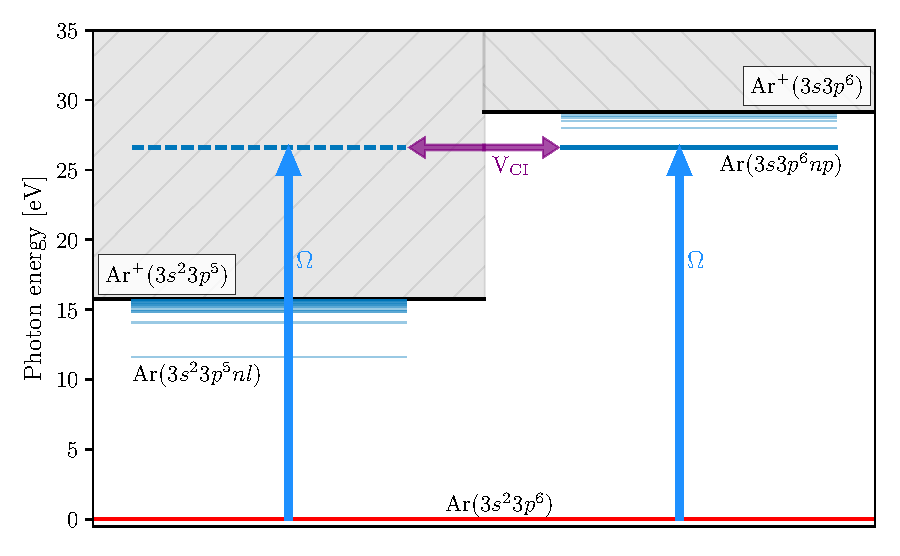
\includegraphics[width=0.8\textwidth]{figures/ATS/fano_level_diagram.pdf}
	\caption{Level diagram of argon showing the effect of autionization states on XUV photoabsorption. There are two possible pathways for ionization with a photon of energy $\Omega$: (1) direct ionization to a continuum state (left side of figure) and (2) excitation to a bound state in the continuum (right side of figure).  In case (2), there is coupling between the bound state and the continuum through the configuration interaction.  This allows for the bound state to decay to the same continuum state as in case (1).  These effect leads to interference between these two pathways.}
	\label{fig:fano_level_diagram}
\end{figure}

The Hamiltonian describing this system can  be written as
\begin{equation}
\label{eqn:hamiltonian}
	\hat{H} = \hat{H_0} + \hat{V},
\end{equation}
where $\hat{H_0}$ is the zeroth order Hamiltonian and $\hat{V}$ is the correlation potential that describes the coupling between the discrete state $\ket{\psi_b}$ and the continuum state $\ket{\psi_\varepsilon}$.  The solutions to the zeroth order Hamiltonian are the continuum and bound states, such that 
\begin{align}
\label{eqn:configurations_hamiltonian}
	\hat{H_0}\ket{\psi_b} &= E_b\ket{\psi_b}\\
	\hat{H_0}\ket{\psi_\varepsilon} &= \varepsilon\ket{\psi_\varepsilon}
\end{align}
where the states $\ket{\psi_b}$ and $\ket{\psi_\varepsilon}$ are orthonormal.  These two solutions to the zeroth order Hamiltonian are referred to as configurations, and the interaction between them is given by $\hat{V}$. The coupling strength between these two configurations is given by the off-diagonal matrix element $V_\varepsilon$, such that
\begin{equation}
\label{eqn:coupling_matrix_element}
	\braket{\psi_\varepsilon|\hat{H}|\psi_b} = \braket{\psi_\varepsilon|\hat{H_0}+\hat{V}|\psi_b} = \braket{\psi_\varepsilon|\hat{V}|\psi_b} = V_\varepsilon.
\end{equation}  
This configuration interaction matrix element $V_\varepsilon$ depends upon the energy $\varepsilon$ and is generally a smooth function of the continuous energy $\varepsilon$.  Furthermore, the configuration interaction only couples different configurations and not within the same configuration.  The means that the diagonal matrix elements of $\hat{V}$ are zero,
\begin{align}
\label{eqn:config_int_diagonal}
	\braket{\psi_\varepsilon|\hat{V}|\psi_\varepsilon} &=0\\
	\braket{\psi_b|\hat{V}|\psi_b} &=0.
\end{align}
Therefore, the diagonal matrix elements of the full Hamiltonian in equation \ref{eqn:hamiltonian} are given by
\begin{align}
	\braket{\psi_\varepsilon|\hat{H}|\psi_\varepsilon} &= \varepsilon\delta(\varepsilon-\varepsilon')\\
	\braket{\psi_b|\hat{H}|\psi_b} &= E_b. 
\end{align}

Armed with these states as a basis, we can now expand an eigenstate of the full Hamiltonian $\hat{H}$.  This entails that the eigenstate $\ket{\Psi_E}$ of energy $E$, which is found by solving the equation
\begin{equation}
	\hat{H}\ket{\Psi_E}=E\ket{\Psi_E},
\end{equation}
can be expanded in this complete basis, such that
\begin{equation}
\label{eqn:eigenstate_expansion}
	\ket{\Psi_E} = a(E)\ket{\psi_b} + \int\diff\varepsilon'b(\varepsilon',E)\ket{\psi_{\varepsilon'}}.
\end{equation}
The physical interpretation of this expansion is that an electron at energy $E$ can originate from either the discrete state $\ket{\psi_b}$ or from the continuous state $\ket{\psi_\varepsilon}$.  The contribution from $\ket{\psi_\varepsilon}$ is direct ionization, and the contribution from $\ket{\psi_b}$ is autoionization (i.e. decay from the bound state $\ket{\psi_b}$ to the continuum).  The relative contributions of these two channels is given by the expansion coefficients $a(E)$ and $b(\varepsilon,E)$.

These expansion coefficients can be solved for and it involves algebra that is described in full detail in Fano's paper \cite{fanoEffectsConfigurationInteraction1961}.  The first step is to evaluate the relationship
\begin{equation}
	\braket{\Psi_E|\hat{H}|\Psi_E} = E
\end{equation}
using the expansion in eqn. \ref{eqn:eigenstate_expansion}.  This results in a system of two equations with the unknown coefficients $a(E)$ and $b(\varepsilon,E)$.  This system can be solved for analytical expressions of the expansion coefficients, and they are given by
\begin{align}
\label{eqn:expansion_coeff_a}
	a(E) &= \frac{\sin\Delta(E)}{\pi V_E}\\
\label{eqn:expansion_coeff_b}
	b(\varepsilon',E) &= \frac{V_{\varepsilon'}}{E-\varepsilon'}a(E)-\delta(\varepsilon'-E)\cos\Delta(E)
\end{align}
where
\begin{align}
\label{eqn:expansion_coeff_delta}
	\Delta(E) &= -\arctan\bigg(\frac{\pi\lvert V_E \rvert^2}{E-E_b-F(E)}\bigg)\\
\label{eqn:expansion_coeff_delta_F}
	F(E) &= \mathrm{PV}\int\diff\varepsilon'\frac{\lvert V_{\varepsilon'}\rvert^2}{E-\varepsilon'} 
\end{align}
and $\mathrm{PV}$ is the Cauchy principal value. The term  $F(E)$ is an energy-dependent shift of the bound state that depends upon the strength of the configuration interaction $\abs{V_{\varepsilon'}}^2$.  This shift can be either positive or negative, depending upon the sign of $\partial_{\varepsilon'}\abs{V_{\varepsilon'}}^2$ at $\varepsilon'=E$, where $\partial_{\varepsilon'}$ is the partial derivative with respect to $\varepsilon'$.  Thus, any change in  $V_{\varepsilon'}$ by an external field will lead to a shift in the resonance position.

Substituting the coefficients in equations \ref{eqn:expansion_coeff_a} and \ref{eqn:expansion_coeff_b} into equation \ref{eqn:eigenstate_expansion} yields
\begin{equation}
	\ket{\Psi_E}=\frac{\sin\Delta(E)}{\pi V_E}\ket{\psi_b}+\frac{\sin\Delta(E)}{\pi V_E}\bigg(\mathrm{PV}\int\diff\varepsilon'\frac{V_{\varepsilon'}}{E-\varepsilon'}\bigg)\ket{\psi_\varepsilon'}-\cos\Delta(E)\ket{\psi_E}.
\end{equation}
This can be further simplified by  introducing a modified discrete state given by
\begin{equation}
	\ket{\Phi} = \ket{\psi_b}+\mathrm{PV}\int\diff \varepsilon'\frac{V_\varepsilon'}{E-\varepsilon'}\ket{\psi_{\varepsilon'}},
\end{equation}
which allows us to express the eigenstate $\ket{\Psi_E}$ as
\begin{equation}
\label{eqn:eigen_with_a_b}
	\ket{\Psi_E}=\frac{\sin\Delta(E)}{\pi V_{E}}\ket{\Phi} - \cos\Delta(E)\ket{\psi_E}.
\end{equation}
Finally, the argument of equation \ref{eqn:expansion_coeff_delta_F} can be written in terms of an important parameter, the reduced energy given by
\begin{equation}
\label{eqn:normalized_eng}
	\epsilon = \frac{E-(E_b+F(E))}{\Gamma(E)/2} = \frac{E-E_\Phi}{\Gamma/2}
\end{equation}
where
\begin{equation}
	\Gamma(E) = 2\pi\abs{V_E}^2\approx\Gamma(E_b)=\Gamma.
\end{equation}
The interpretation of the modified bound state $\ket{\Phi}$ is that the configuration interaction is mixing the original discrete state $\ket{\psi_b}$ and the continuum states $\ket{\psi_\varepsilon'}$. So, for an energetic window near $E=E_\Phi$, one can consider the resonance energy to be $E_b$ and the resonance linewidth to be $\Gamma$.  Since $\Gamma=2\pi\abs{V_E}^2$, the resonance linewidth and the natural lifetime $h/\Gamma$ are directly related to the strength of the coupling between bound states and continuum states though the configuration interaction. Therefore, stronger (weaker) coupling would lead to faster (slower) decay from bound to continuum states, respectively.  From this, it can be seen that an external field that  is able to modify the strength of the configuration interaction, then that will lead to a change in the linewidth and position of the resonance.

Now that the eigenstates of the Hamiltonian $\hat{H}$ have been expanded, we will turn our attention to the photoabsorption spectrum.  In the original experiments done by Beutler, a sharp, asymmetric absorption profile was seen in the photoabsorption spectrum of noble gas atoms in the XUV \cite{beutlerUeberAbsorptionsserienArgon1935}.  From the expanded eigenstate given in equation \ref{eqn:eigen_with_a_b}, we can begin see how this asymmetric absorption profile might arise.  The coefficients in the expansion are proportional to sine and cosine functions of the reduced energy $\epsilon$, and, since they are odd and even functions of $\epsilon$, this will lead to constructive and destructive interference on either side of the resonance.  It is precisely this effect that will give rise to the asymmetric absorption lineshape.

To derive the photoabsorption spectrum, we will consider a transition from the ground state of the atom $\ket{g}$ by a XUV photon of energy $\Omega$.  This can be described through the use of the dipole transition operator
\begin{equation}
\label{eqn:dipole}
	\hat{D}=-e\mathbf{\hat{r}}\cdot\mathbf{E}_{XUV}(t)
\end{equation}
where $\mathbf{E}_{XUV}(t)$ is the electric field of the XUV.  Using this operator, the transition probability is given by the matrix element
\begin{equation}
\label{eqn:transition_me}
	\begin{aligned}
		\braket{\Psi_E|\hat{D}|g} &= \frac{1}{\pi V^*_{E}}\sin\Delta(E)\braket{\Phi|\hat{D}|g}-\cos\Delta(E)\braket{\psi_E|\hat{D}|g}\\
		&= \cos\Delta(E)\braket{\psi_E|\hat{D}|g}\Bigg[\tan\Delta(E)\frac{1}{\pi V^*_E}\frac{\braket{\Phi|\hat{D}|g}}{\braket{\psi_E|\hat{D}|g}} -1\Bigg].
	\end{aligned} 
\end{equation}
At this point, we can now introduce the well-known and important $q$ parameter, given by
\begin{equation}
\label{eqn:q-parameter}
	q(E) = \frac{1}{\pi V^*_E}\frac{\braket{\Phi|\hat{D}|g}}{\braket{\psi_E|\hat{D}|g}}\approx q(E_b)=q.
\end{equation}
The $q$ parameter describes the asymmetry of the resonance, and it is related to the ratio of transitions to the modified bound state $\ket{\Phi}$ and the continuum states $\ket{\psi_E}$.  Combining equations \ref{eqn:transition_me}, \ref{eqn:q-parameter}, and \ref{eqn:expansion_coeff_delta}, we arrive at
\begin{align}
	\braket{\Psi_E|\hat{D}|g} &=-\cos\Delta(E)\braket{\psi_E|\hat{D}|g}\Bigg[\frac{\pi\abs{V_E}^2}{E-(E_b+F(E))}q+1\Bigg]\\
	&=-\cos\Delta(E)\braket{\psi_E|\hat{D}|g}\Bigg[\frac{\Gamma/2}{E-(E_b+F(E))}q+1\Bigg],
\end{align}
and this can be further simplified using the reduced energy $\epsilon$, which yields
\begin{align}
	\braket{\Psi_E|\hat{D}|g} &= -\braket{\psi_E|\hat{D}|g}\cos\Delta(E)\bigg(\frac{q}{\epsilon}+1\bigg)\\
\label{eqn:fano_matirx_elements}
	\braket{\Psi_E|\hat{D}|g} &= \braket{\psi_E|\hat{D}|g}\frac{q+\epsilon}{\epsilon+i}.
\end{align}
Finally, using this relationship the ratio of transition probabilities can be calculated and leads to the well known Fano lineshape,
\begin{equation}
\label{eqn:transition_prob_ratio}
	\frac{\abs{\braket{\Psi_E|\hat{D}|g}}^2}{\abs{\braket{\psi_E|\hat{D}|g}}^2}=\frac{(q+\epsilon)^2}{\epsilon^2 + 1}.
\end{equation}
This ratio is proportional to the photoabsorption cross section, and is plotted for various $q$ parameters in figure \ref{fig:cross_sec_and_phase}.  As can be seen, the lineshape's symmetry dramatically depends upon the $q$ parameter, and the cross section even goes to zero at different energies, depending upon $q$. This is a direct consequence of the destructive interference from the configuration states, as was predicted earlier in the derivation. Additionally, the spectral phase of the Fano profile can also be extracted, given by 
\begin{equation}
	\theta(\epsilon)=\arg\bigg[\frac{q+\epsilon}{\epsilon+i}\bigg],
\end{equation}
and is plotted in figure \ref{fig:cross_sec_and_phase} (b).  For increasing $\epsilon$, the phase increases until $\epsilon=-q$ when there is a $\pi$ phase jump, and thereafter the phase continues to increase until is asymptotically approaches its original value.
\begin{figure}
	\centering
	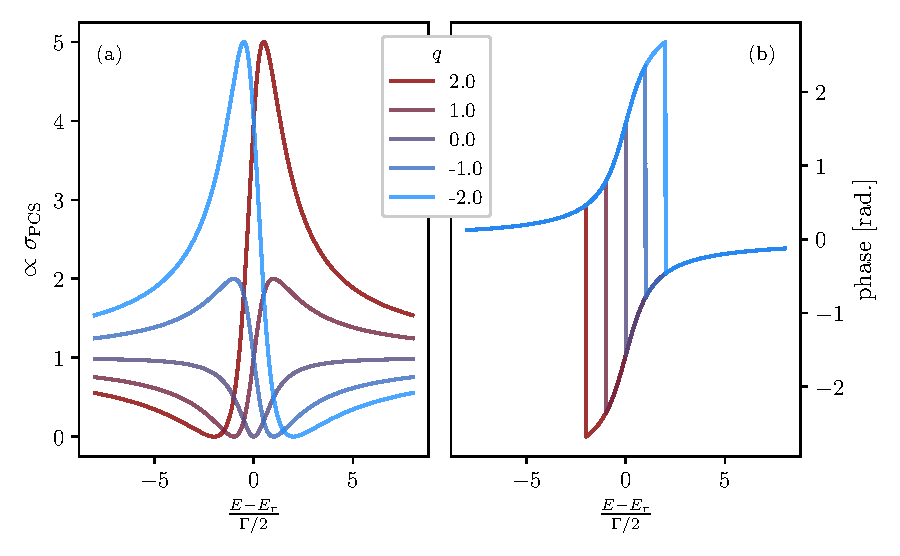
\includegraphics[width=0.8\textwidth]{figures/ATS/cs_phase.pdf}
	\caption{(a) Calculation of the photoabsorption cross section near a resonance for the listed $q$ parameters.  The change from symmetric to asymmetric profiles can be seen as the $q$ parameter is varied. Maximum and minimum in cross section occus at $\epsilon=1/q$ and $\epsilon=-q\Gamma^2/4$, respectively. (b) Calculation of the phase across the resonance for different $q$ parameter. The $\pi$ phase jump clearly depends on $q$, and it occurs when $\epsilon=-q$ and not at the resonance energy $E_r$. Calculations based on U. Fano's original work \cite{fanoEffectsConfigurationInteraction1961}.}
	\label{fig:cross_sec_and_phase}
\end{figure}

Experimentally the photoabsorption cross section is generally fit to the form
\begin{equation}
\label{eqn:sigma_pcs}
	\sigma_\mathrm{PCS}=\sigma_a\frac{(q+\epsilon)^2}{\epsilon^2+1}+\sigma_{NR}
\end{equation}
where $\sigma_a$ scales the strength of the Fano profile and $\sigma_{NR}$ is  a non-resonant cross section that is included to account for absorption from  other continuum states that might be present.  



\subsection{Autoionization in the time domain}
\label{sec:time_dependent_autoionization}
%
%!!!!!!!!!!!!!!!!!!!!!!!!!!!!!!!!!!!!!!!!!!!!!!!!!!!!!!!!!!!!!!!!!!!!!!!!!!!!!!!!!
%!!!!!!!!!!!!!!!!!!!!!!!!!!! ATOMIC UNITS !!!!!!!!!!!!!!!!!!!!!!!!!!!!!!!!!!!!!!!!
%!!!!!!!!!!!!!!!!!!!!!!!!!!!!!!!!!!!!!!!!!!!!!!!!!!!!!!!!!!!!!!!!!!!!!!!!!!!!!!!!!
%

Up until this point, Fano resonances have been discussed in a time-independent manner in the frequency domain.  However, one would ideally like to describe these autoionizing resonances in the time domain, as that will lend itself to the experiments described herein. This description was primarily done by W.-C. Chu and C.D. Lin \cite{chuTheoryUltrafastAutoionization2010}, and it has been used to interpret many ATS experiments  \cite{kaldunExtractingPhaseAmplitude2014,ottLorentzMeetsFano2013,ottReconstructionControlTimedependent2014, stoossRealTimeReconstructionStrongFieldDriven2018}.  The basic assumption that is made in this treatment is that the XUV pulse that excites from the ground state to the Fano resonance is a Dirac-$\delta$ function in time, $\mathbf{E}_{XUV}=E_0\delta(t)\mathbf{z}$.  This impulsive excitation is generally a reasonable  approximation for an attosecond XUV pulse that is shorter in duration than the typical lifetimes of these resonances.  From this assumption, it is possible to analytically describe the dipole response of the system in the time domain.


The derivation of the dipole response follows naturally from the theory described in the previous section. Assuming that the XUV impulsively excites at $t=0$ from the ground state $\ket{g}$ to the bound and continuum states $\ket{\psi_b}$ and $\ket{\psi_\varepsilon}$, the wave function for times $t>0$ can be in the configuration states, such that
\begin{equation}
\label{eqn:wvfnc_expansion}
	\ket{\Psi(t)}=e^{-i\varepsilon_gt}\ket{g}+c_b(t)\ket{\psi_b}+\int c_\varepsilon(t)\ket{\psi_\varepsilon}\diff \varepsilon.
\end{equation}
Since the configuration states $\ket{\psi_b}$ and $\ket{\psi_\varepsilon}$ are not eigenstates of the total Hamiltonian, the expansion coefficients $c_b$ and $c_\varepsilon$ are explicitly time dependent. The evolution of these coefficients is governed by the Time-Dependent Schr{\"o}dinger Equation (TDSE)
\begin{equation}
\label{eqn:tdse}
	i\frac{\partial}{\partial t}\ket{\Psi(t)}=\hat{H}\ket{\Psi(t)},
\end{equation}
and using this equation, the time dependence of the expansion coefficients can be expressed as the coupled differential equations given by
\begin{equation}
\label{eqn:coupled_pde}
	\begin{aligned}
		\frac{\partial c_{\varepsilon}}{\partial t} &= -iV_\varepsilon c_b(t)-i\varepsilon c_\varepsilon(t)\\
		\frac{\partial c_b}{\partial t} &= -i\varepsilon_r c_b(t)-iV_\varepsilon \int c_\varepsilon(t) \diff \varepsilon.
	\end{aligned}
\end{equation}
Assuming the initial values $c_b^{(0)}$ and $c_\varepsilon^{(0)}$ are known, then the solutions to equations \ref{eqn:coupled_pde} are given by
\begin{equation}
\label{eqn:coefficients}
	\begin{aligned}
		c_b(t) &= c_b^{(0)}\bigg(1-\frac{i}{q}\bigg)e^{-i\varepsilon_r}e^{-\frac{\Gamma}{2}t}\\
		c_\varepsilon(t) &= \frac{c_\varepsilon^{(0)}}{\epsilon + i}e^{-i\varepsilon_r t}\bigg[ (q+\epsilon)e^{-i(E-E_r)t}-(q-i)e^{-\frac{\Gamma}{2}t}\bigg],
	\end{aligned}
\end{equation}
where, as in the previous section, $q=c_b^{(0)}/(\pi V c_\varepsilon^{(0)})$, $\Gamma=2\pi\rvert V \lvert^2$, and $\epsilon=(\varepsilon-\varepsilon_r)/(\Gamma/2)$. 


\begin{figure}
	\centering
	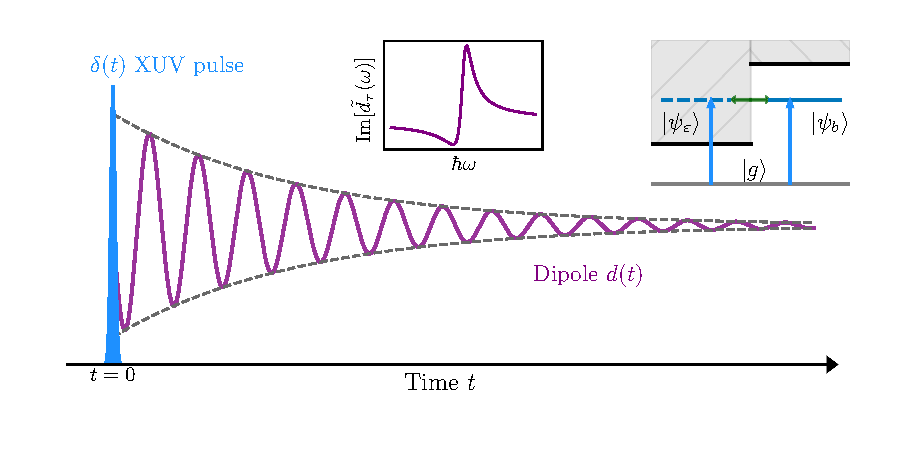
\includegraphics[width=1.0\textwidth]{figures/ATS/dipole_sketch.pdf}
	\caption{Illustration of the dipole moment after a $\delta(t)$ excitation pulse. Dipole is shown for a phase shift of $\varphi=-1.2\pi$ (purple curve) and $\varphi=0$ (dashed gray curve), and the central inset shows the line shape for these two phase shifts.}
	\label{fig:dipole_sketch}
\end{figure}

With the time dependent wave function now in hand, the induced dipole $d(t)$ can now be calculated for $t>0$ by evaluating  $d(t)=\braket{\Psi(t)|z|\Psi(t)}$.  Using equations \ref{eqn:wvfnc_expansion} and \ref{eqn:coefficients}, this gives
\begin{equation}
\label{eqn:dip}
	\begin{aligned}
		d(t)&=c_b(t)e^{-i\varepsilon_g t}\braket{\psi_b|z|g}^* + \int c_\varepsilon(t)e^{i\varepsilon_g t}\braket{\psi_\varepsilon|z|g}^* + c.c.\\
		&=c_b^{(0)}\braket{\psi_b|z|g}^*e^{-i\Omega_r t}\Bigg[\bigg(1-\frac{i}{q}\bigg)e^{-\frac{\Gamma}{2}t}+ \frac{1}{(\pi V q)^2}\int \frac{(q+\epsilon)e^{-i\frac{\Gamma}{2}\epsilon t}-(q-i)e^{\frac{\Gamma}{2}t}}{\epsilon+i}\diff\varepsilon\Bigg] + c.c.,
	\end{aligned}
\end{equation}
where $\Omega_r=E_r-E_g$ is the resonance photon energy.  The complex conjugate term in equation \ref{eqn:dip} is a counter-rotating term, and by invoking the rotating wave approximation, it can be dropped.  Equation \ref{eqn:dip} can further be evaluated to give
\begin{equation}
	\begin{aligned}
	d(t) &= c_b^{(0)}\braket{\psi_b|z|g}^*e^{-i\Omega_r t}\frac{1}{q^2}\Bigg[q(q-i)e^{-\frac{\Gamma}{2}t}+\frac{2}{\pi\Gamma}\int \frac{(q+\epsilon)e^{-i\frac{\Gamma}{2}\epsilon t}-(q-i)e^{\frac{\Gamma}{2}t}}{\epsilon+i}\diff\varepsilon\Bigg]\\
	&= c_b^{(0)}\braket{\psi_b|z|g}^*e^{-i\Omega_r t}\frac{1}{q^2}\Bigg[q(q-i)e^{-\frac{\Gamma}{2}t} + \frac{1}{\pi} \int e^{-i\frac{\Gamma}{2}\epsilon t}\diff\epsilon + \frac{q-i}{\pi}\int \frac{e^{-i\frac{\Gamma}{2}\epsilon t} - e^{-\frac{\Gamma}{2}t}}{\epsilon+i} \diff\epsilon\Bigg]\\
	&=c_b^{(0)}\braket{\psi_b|z|g}^*e^{-i\Omega_r t}\frac{1}{q^2} \Bigg[ q(q-i)e^{-\frac{\Gamma}{2}t}+ \frac{4}{\Gamma}\delta(t) + \frac{q-i}{\pi}e^{-\frac{\Gamma}{2}t}2\pi i + \frac{q-i}{\pi}e^{-\frac{\Gamma}{2}t}\pi i \Bigg]\\
	&=c_b^{(0)}\braket{\psi_b|z|g}^*\frac{1}{q^2}\bigg[ \frac{4}{\Gamma}\delta(t)+(q-i)^2e^{-i\Omega_r t}e^{-\frac{\Gamma}{2}t}\bigg].
	\end{aligned}
\end{equation}
If we assume that $\braket{\psi_b|z|g}$ is real and the expansion coefficient is $c_b^{(0)}$ purely imaginary, then we can finally arrive at the form of the dipole that is reported in \cite{chuTheoryUltrafastAutoionization2010,ottLorentzMeetsFano2013,kaldunFanoResonancesTime2014},
\begin{equation}
\label{eqn:dipole_time_domain}
	d(t)\propto i\bigg[ 2\delta(t) + \frac{\Gamma}{2}(q-i)^2 e^{-i\Omega_r t}e^{\frac{\Gamma}{2}t} \bigg].
\end{equation}
This form of the dipole can be understood intuitively as arising naturally from the two interfering processes that are occurring: direct ionization to the continuum and decay from a discrete state to the continuum with a lifetime of $\hbar/\Gamma$.  The first $\delta$-function in equation \ref{eqn:dipole_time_domain} represents direct ionization, and the second term represents decay from the discrete state.  A schematic of the dipole after an impulsive XUV pulse is shown in  figure \ref{fig:dipole_sketch}.  To demonstrate that this formulation of the dipole in the time domain is compatible with Fano's original derivation, the photoabsorption cross section can be evaluated by
\begin{equation}
\begin{aligned}
	\sigma&=\frac{2\omega}{\epsilon_0 c}\mathrm{Im}\bigg[\frac{\tilde{d}(\omega)}{\tilde{E}(\omega)}\bigg]\propto \mathrm{Im}\bigg[\int_{-\infty}^{\infty} d(t) e^{i\omega t} \diff t\bigg]\\
	&\propto\mathrm{Re}\bigg[1+\frac{\Gamma}{2}(q-i)^2\int_0^\infty e^{-\frac{\Gamma}{2}t}e^{i(\omega-\Omega_r)t}\bigg]\\
	&\propto\mathrm{Re}\bigg[1 + \frac{(q-i)^2}{1-i\epsilon}\bigg]\\
	& \propto \frac{(q+\epsilon)^2}{\epsilon^2 +1}.
\end{aligned}
\end{equation}
This is exactly the cross section in equation \ref{eqn:sigma_pcs} that was derived previously.

\begin{figure}
	\centering
	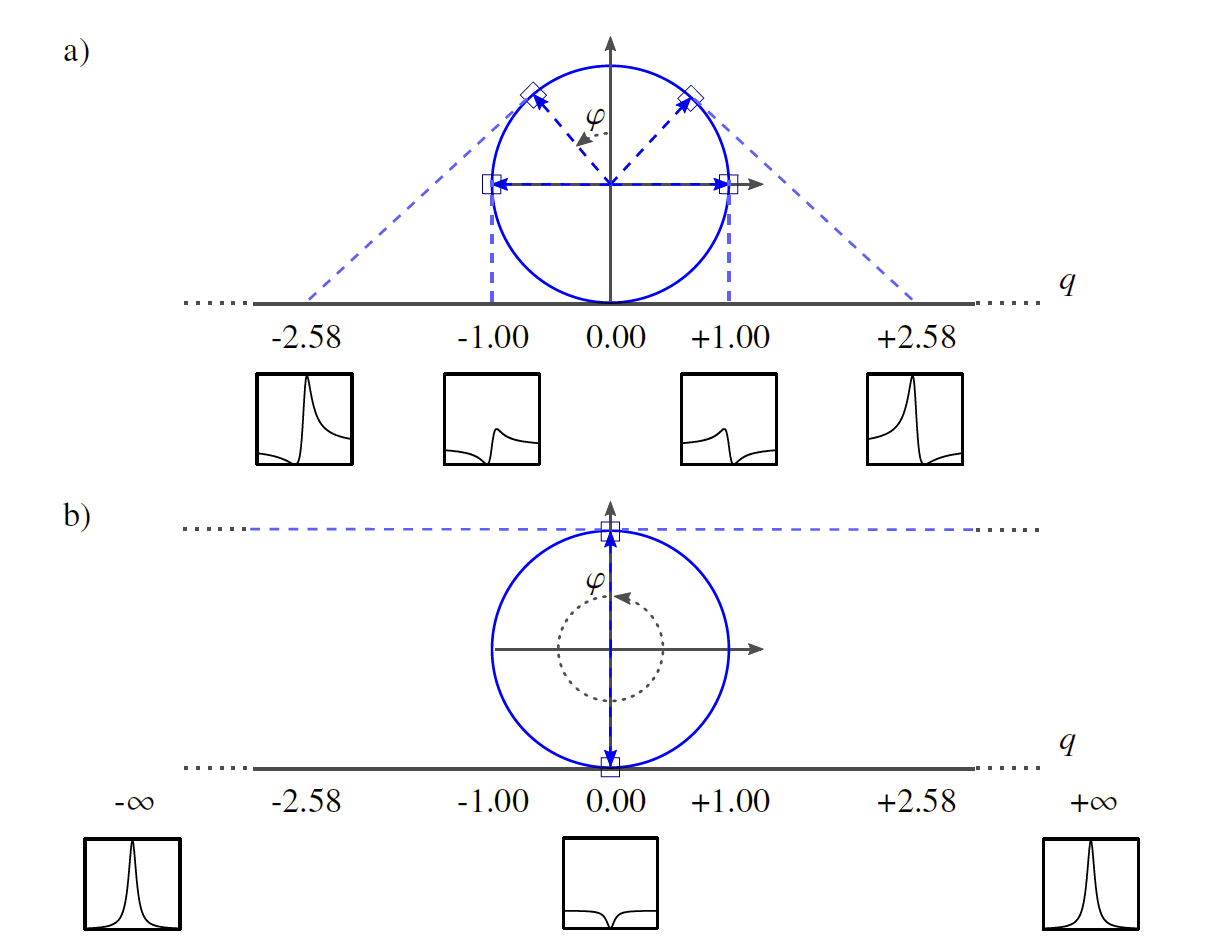
\includegraphics[width=0.8\textwidth]{figures/ATS/Kaldun.png}
	\caption{Illustration of the mapping between the Fano $q$ parameter and the phase shift $\varphi$ of the dipole. (a) Phase shift $\varphi$ is shown as a counter-clockwise rotation of a vector on the unit circle. Dashed tangent lines for a given $\varphi$ show the mapping to the value $q(\varphi)$ along the $q$-axis. (b) Shows the special cases of a Lorentzian line shape ($q\rightarrow\pm\infty$, $\varphi=0$) and a window resonance ($q=0$, $\varphi=\pi$).  Adapted from \cite{kaldunFanoResonancesTime2014}.}
	\label{fig:q_to_phi}
\end{figure}

The complex coefficient in front of the second term of equation \ref{eqn:dipole_time_domain} arises from the configuration interaction, and its influence on the dipole can be elucidated by expressing it as an exponential,
\begin{equation}
	(q-i)^2 = (q^2+1)e^{i\varphi(q)}
\end{equation} 
where the phase is given by
\begin{equation}
	\varphi(q)=2\arg(q-i).
\end{equation}
Substituting this form into the dipole in equation \ref{eqn:dipole_time_domain} gives
\begin{equation}
\label{eqn:dipole_time_domain_phasse_shift}
	d(t)\propto i\bigg[ 2\delta(t) + \frac{\Gamma}{2}(q^2+1)e^{i\varphi(q)}e^{-i\Omega_r t}e^{\frac{\Gamma}{2}t} \bigg].
\end{equation}
By expressing the dipole this way, it is clear that the autoionization from the discrete state is phase shifted relative to the instantaneous response (direct ionization).  Furthermore, in section \ref{sec:og_fano} it was established that the $q$ parameter determines the line shape of the photoabsorption cross section ($\sigma\propto\mathrm{Im}[\tilde{d}(\omega)]$). This fact, combined with the correspondence between $\varphi$ and $q$, means that the line shape of the Fano resonance is determined by the phase shift of the dipole response.  Thus, if one can experimentally introduce a phase shift of the dipole response then it is possible to control the absorption process.  In fact, if one has sufficient control over the dipole phase shift then it is possible to continuously change the line shape from symmetric to asymmetric and vice versa.  This mapping of $q$ parameter and the phase shift $\varphi$ and its affect on the line shape is shown in figure \ref{fig:q_to_phi}.


\section{Dipole Control Model}

Now that the relationship between the dipole and the absorption line shape has been established in the time domain, we would like to establish a method to control and modify the dipole.  This will be done by introducing an IR probe/dressing pulse at a variable time delay $\tau$.  This IR pulse will lead to a modification of the dipole that can be modeled analytically for certain assumptions. This model is referred to as the dipole control model (DCM), and it was originally formulated by A. Bl{\"a}tterman, et al \cite{blattermannImpulsiveControlAtomic2016, blattermannTwodimensionalSpectralInterpretation2014, kaldunFanoResonancesTime2014}. In a similar manner to the previous section, a key assumption that must be made in this model is that, in addition to the XUV pulse, the IR pulse must be a $\delta$-function in time.  This is generally only a reasonable approximation if the pulse duration is much shorter than the lifetime $\hbar/\Gamma$.  These assumptions will be questionable for the experiments discussed in this chapter, however this model will allow for an understanding of the features that will be seen in the data shown later.  


A schematic of the physical situation considered for the DCM is shown in figure \ref{fig:dipole_sketch_dressing}.  A XUV pulse at $t=0$ induces a dipole $d(t)$, and an IR pulse perturbs the dipole after a time delay of $\tau$. The $\delta$-function nature of both pulses means that there are three distinct temporal regions to consider.  The first is $t<0$, and in this region, the dipole response is zero because the XUV pulse hasn't yet populated the excited state. For the region between the two pulses, the dipole is allowed to freely evolve in time, as was derived in \ref{eqn:dipole_time_domain_phasse_shift}. Thus, the dipole response here is just simply
\begin{equation}
	d(0<t<\tau)= f_0(t)\propto i\bigg[ c\delta(t) + \frac{\Gamma}{2}(q-i)^2 e^{-i\Omega_r t}e^{\frac{\Gamma}{2}t} \bigg].
\end{equation}
At $t=\tau$, the dressing field will interact with the system through resonant and non-resonant processes which will modify the dipole response.  However, since the dressing field is infinitesimally short in duration, the system will again freely evolve in time for times after $\tau$, but the dressing field is assumed to have modified the dipole amplitude and phase.  Therefore, in the third temporal region of $t>\tau$, the dipole response is given by
\begin{equation}
	d(t>\tau) = A f_0(t)
\end{equation}
where $A$ is the complex perturbation to the dipole response induced by the dressing pulse. By combing the dipole response for the three temporal regions into a single piece-wise function, we arrive at
\begin{equation}
	d_\tau(t)=
	\begin{cases}
		0 & t<0\\
		f_0(t) & 0<t<\tau\\
		A(\tau)f_0(t) & t>\tau.
	\end{cases}
\end{equation}

In general, $A$ is a complex quantity that can be explicitly dependent upon $\tau$ or $\omega$, and it can  be used to describe both resonant and non-resonant processes.  For example, a decrease of the amplitude of $A$ can be used to represent ionization of the excited state by the dressing field, whereas the phase can be used to describe a ponderomotive shift of energy levels by the dressing field.  To describe these non-resonant processes, it can be assumed that $A$ takes the form of $A=a_1e^{i\phi_1}$.  To describe a resonant process such as coupling of excited states, $A$ takes the form $A=1+a_2e^{i(\Delta\omega\tau+\phi_2)}$ where $\hbar\omega$ is the separation of the states.  This form is motivated by the results of perturbation theory (see appendix \ref{chap:Perturbation_theory}).  These two primitive forms can be linearly combined into
\begin{equation}
	A=a_1e^{i\phi_1}(1+a_2e^{i(\Delta\omega\tau+\phi_2)}).
\end{equation}
In general, all of these quantities can be explicitly dependent upon $\tau$ and $\omega$, however they are independent of $t$.

Armed now with the dipole in the time domain, it is possible now to calculate the cross section from the dipole in the frequency domain.  The spectral dipole is given by the Fouier transform, and it can be conveniently calculated
\begin{equation}
	\begin{aligned}
	\tilde{d}_\tau(\omega,\tau)&=\int_{-\infty}^{\infty} d_\tau(t,\tau)e^{i\omega t}\diff t\\
	&=\int_0^\tau f_0(t)e^{i\omega t}\diff t + \int_\tau^\infty A(\tau)f_0(t)e^{i\omega t}\diff t\\
	&=\int_0^\tau i\bigg[ 2\delta(t) + \frac{\Gamma}{2}(q-i)^2 e^{-i\Omega_r t}e^{\frac{\Gamma}{2}t} \bigg]e^{i\omega t}\diff t \\ & + A(\tau)\int_\tau^\infty i\bigg[ 2\delta(t) + \frac{\Gamma}{2}(q-i)^2 e^{-i\Omega_r t}e^{\frac{\Gamma}{2}t} \bigg]e^{i\omega t}\diff t\\
	&=i-\gamma(q-i)^2\frac{1-(1-A(\tau))e^{-\gamma\tau -i\delta\tau}}{\delta+i\gamma}
	\end{aligned}
\end{equation}
where $\gamma = \Gamma/2$ and $\delta=\omega-\omega_r$.

\begin{figure}
	\centering
	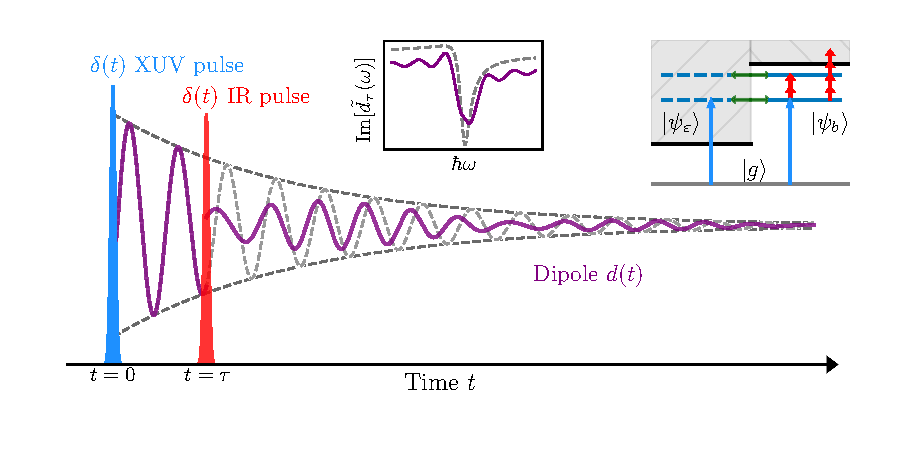
\includegraphics[width=1.0\textwidth]{figures/ATS/dipole_sketch_dressing.pdf}
	\caption{Incomplete}
	\label{fig:dipole_sketch_dressing}
\end{figure}




\begin{figure}
	\centering
	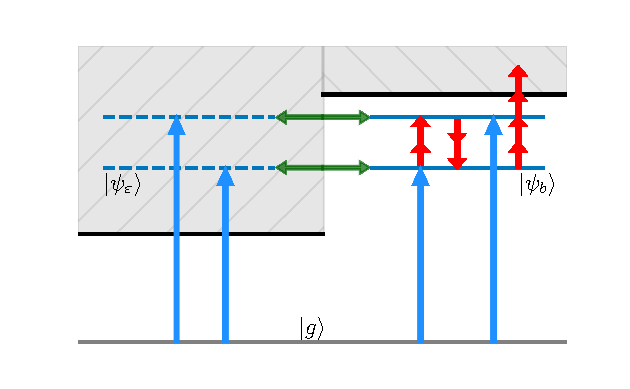
\includegraphics[width=0.7\textwidth]{figures/ATS/level_diagram_sketch.pdf}
	\caption{Level diagram showing the influence of the IR dressing pulse on a series of Fano resonances. Generally, the IR field can either couple different resonances or directly ionize from the discrete state. Coupling is shown here as a two-photon transition between discrete states, and direct ionization from a discrete state is shown as a multiphoton process.  Green arrows represent the configuration interaction coupling the discrete states to the continuum.}
	\label{fig:level_diagram_dressing}
\end{figure}


\begin{figure}
	\centering
	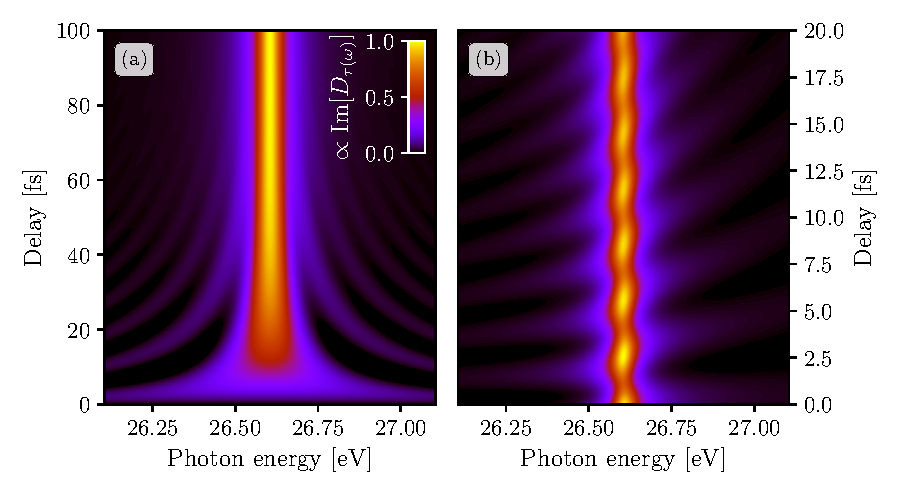
\includegraphics[width=1.0\textwidth]{figures/ATS/resonant_vs_non_resonant.pdf}
	\caption{Incomplete}
	\label{fig:res_vs_non_res}
\end{figure}

\begin{figure}
	\centering
	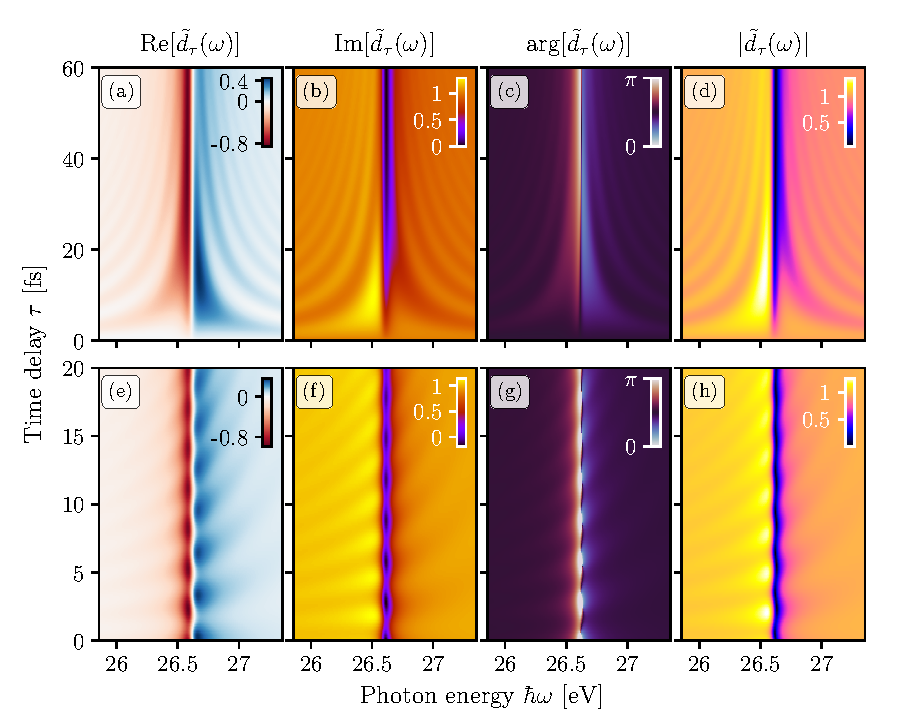
\includegraphics[width=1.0\textwidth]{figures/ATS/dipole_components.pdf}
	\caption{$\varphi_1=0$}
	\label{fig:dip_components}
\end{figure}

\begin{figure}
	\centering
	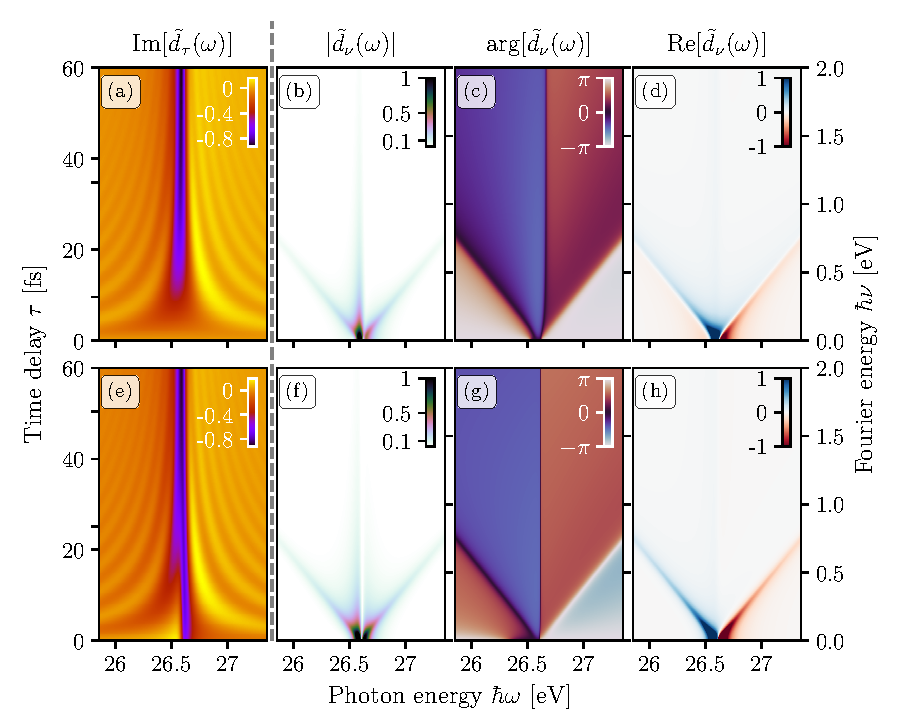
\includegraphics[width=1.0\textwidth]{figures/ATS/DCM_non_res_high_low.pdf}
	\caption{$\phi_0=4p$ $a_1=0,\phi_1=0$, $a_1=0.8,\phi_1=\pi/2$}
	\label{fig:non_res_high_low}
\end{figure}

\begin{figure}
	\centering
	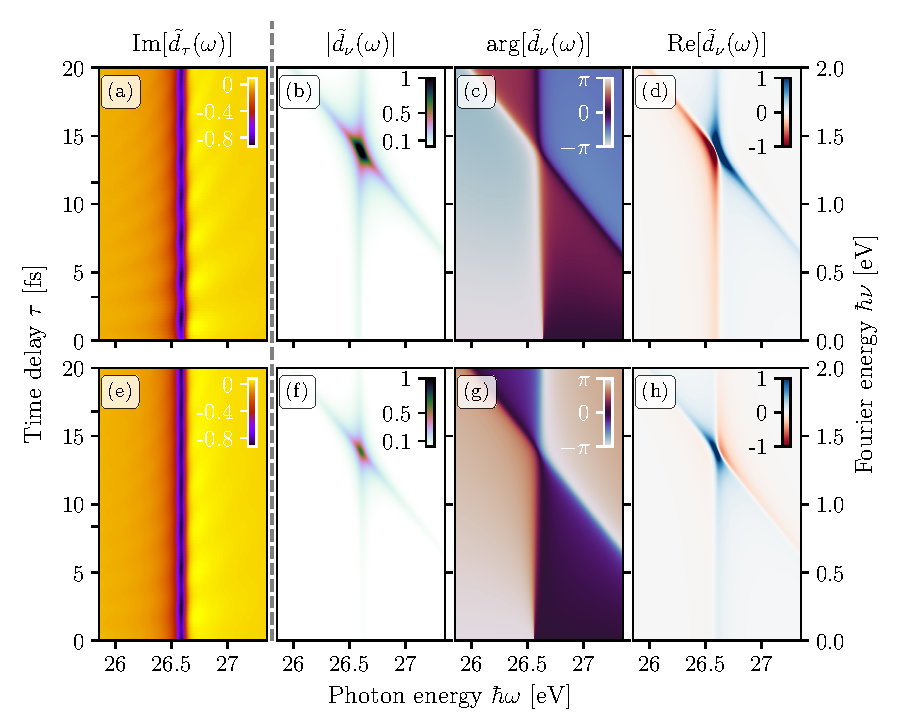
\includegraphics[width=1.0\textwidth]{figures/ATS/DCM_res_high_low.pdf}
	\caption{$\phi_0=4p$ $a_1=0,\phi_1=0$, $a_1=0.8,\phi_1=\pi/2$}
	\label{fig:res_high_low}
\end{figure}

\section{Strong-field Transient Absorption in Argon}
\label{sec:ATS_ar}

\subsection{Experimental setup}
\label{sec:ATS_ar_exp_setup}


\begin{table}[]
	\centering
	\begin{tabular}{lcccc}
		\hline\hline
		\multicolumn{1}{c}{} & $\Delta E$ [eV]   & $\Gamma$ [meV]   & $q$         & $\rho^2$     \\ \hline
		$3s3p^64p$              & 26.605 & 80.2(7) & -0.286(4) & 0.840(3) \\
		$3s3p^65p$              & 27.994 & 28.5(8) & -0.177(3) & 0.848(3) \\
		$3s3p^66p$              & 28.509 & 12.2(3) & -0.135(9) & 0.852(9) \\
		$3s3p^67p$              & 28.757 & 6.6(1)  & -0.125(4) & 0.846(9) \\
		$3s3p^68p$              & 28.898 & 4.5(2)  & -0.132(4) & 0.77(2)  \\ \hline\hline
	\end{tabular}
	\caption{Paramters of the $3s3p^6np$ Fano resonances in argon. These values were extracted from experimental cross sections, see \cite{caretteMulticonfigurationalHartreeFockClosecoupling2013, wuElectronimpactStudyValence1995, berrahAngulardistributionParametersAndRmatrix1996}.}
	\label{table:fano_params}
\end{table}

\begin{figure}
	\centering
	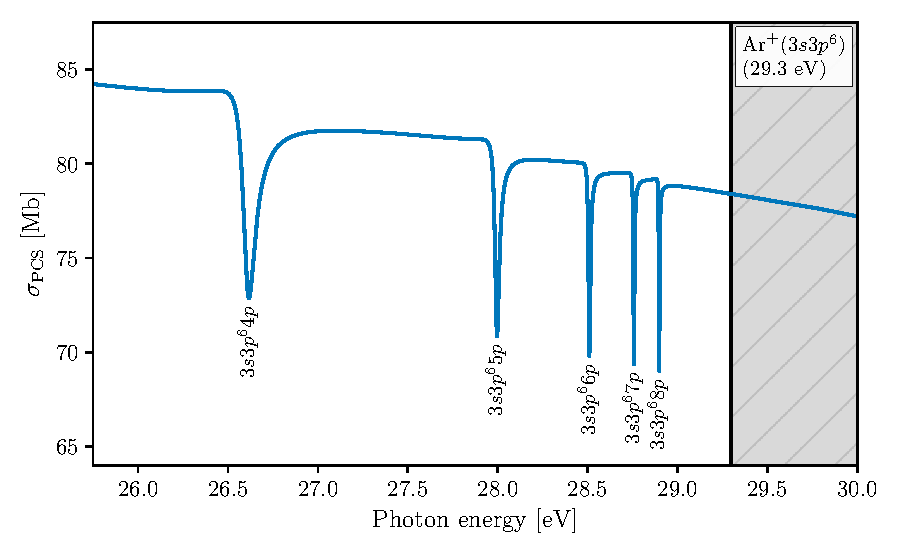
\includegraphics[width=0.8\textwidth]{figures/ATS/fano_GS.pdf}
	\caption{Photoabsorption cross section of the Argon $3s3p^6np$ Fano resonances (blue curve), with only resonances up to $n=8$ shown.  Grey shaded area indicates the energetic region above the $\mathrm{Ar}^+(3s3p^6)$ ionization threshold. Values used to calculate this cross section are shown in Table \ref{table:fano_params}.}
	\label{fig:fano_gs_pcs}
\end{figure}

\begin{figure}
	\centering
	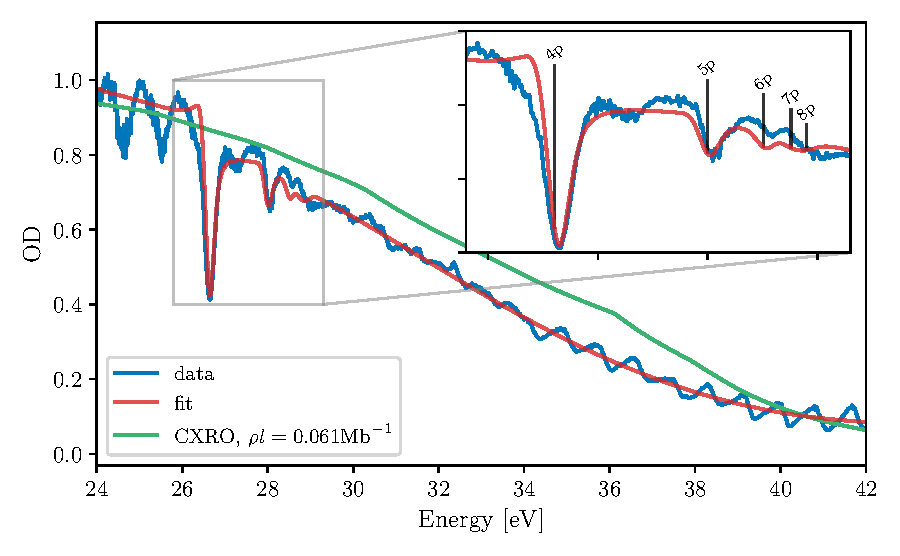
\includegraphics[width=0.8\textwidth]{figures/ATS/fano_fit.pdf}
	\caption{Incomplete}
	\label{fig:fano_fit}
\end{figure}

\subsection{Results}
\label{sec:ATS_ar_results}

\section{Conculsion}
\label{sec:ATS_conclusion}

